%% Example data sheet
%% Feel free to modify and use this file for any purpose, under
%% either the LaTeX Project Public License or under public domain.

% Options here are passed to the article class.
% Most common options: 10pt, 11pt, 12pt
\documentclass[10pt]{datasheet}

% Input encoding and typographical rules for English language
\usepackage[utf8]{inputenc}
\usepackage[english]{babel}
\usepackage[english]{isodate}
\usepackage{float}
% tikz is used to draw images in this example, but you can
% also use \includegraphics{}.
\usepackage{tikz}
\usepackage{pgfplots}
\usepackage{circuitikz}
\usepackage{ltablex}   % makes tabularx-style X columns work inside longtable
\usepackage{pdflscape}

\keepXColumns
\usetikzlibrary{calc}
\usepackage[justification=centering]{caption}
% These define global texts that are used in headers and titles.
\title{Lumostep Data Sheet}
\author{Lab 03 Group 2}
\date{May 2026}
\revision{Revision 1}
\companylogo{\Huge $\nabla$ Lab 03 Group 2}

\begin{document}
\maketitle

\section{Features}

\begin{itemize}
\item{OLED touch screen}
\item{Reliable step tracking and pace identification}
\item{Accelerometer's self-testing}
\item{USB-C powered, charging and programming}
\item{Integrated 500mAh rechargeable lipo}
\item{Built-in apps for entertainment}
\item{Wearable design}
\item{Calories tracking}

\end{itemize}
\begin{figure}[b!]
    \centering
        \rotatebox{90}{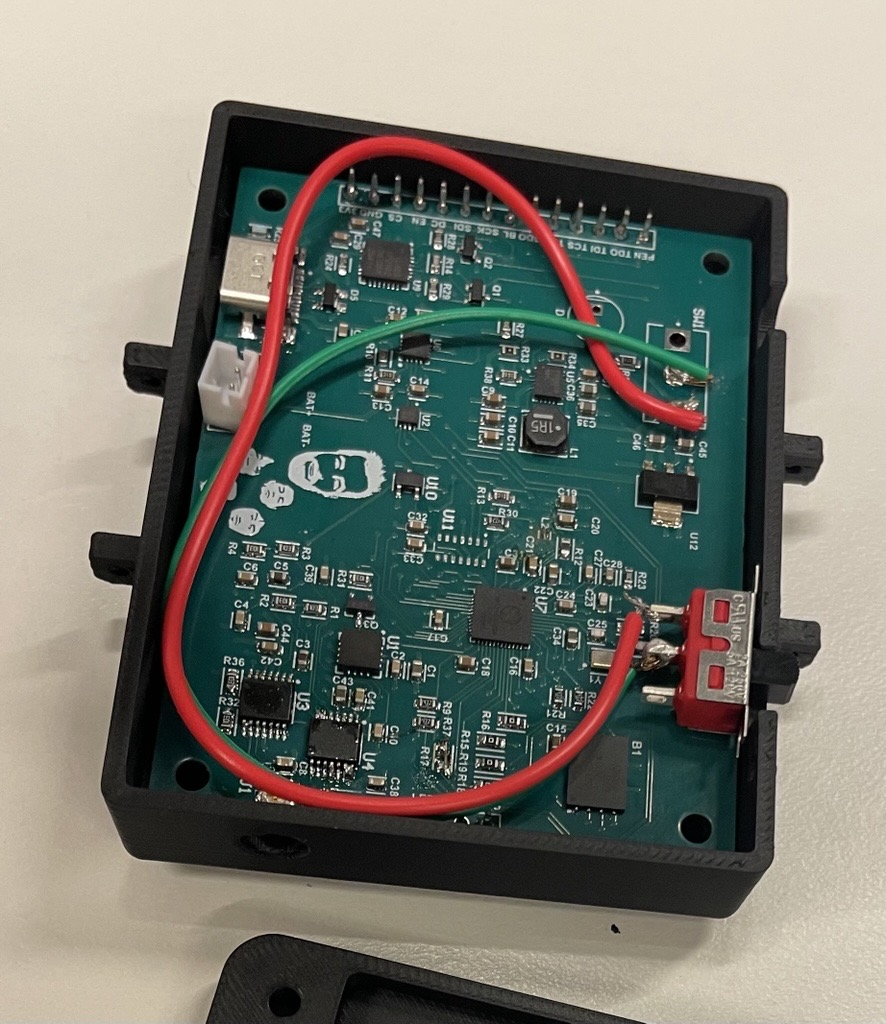
\includegraphics[width=0.35\textwidth]{PCB.jpg}}     
    \caption{Lumostep Teardown}
\end{figure}

\section{Applications}

\begin{itemize}
\item{Fitness band}
\item{Hand-held gaming device}
\item{Stop watch}
\item{General Dev Board}
\end{itemize}
% Switch to next column
\vfill\break

\section{General Description}
Lumostep is an ESP-32 based, wearable fitness band, utilizing a 2.4 inch touch screen for graphics and collecting user inputs. The core functionalities are built around an ADXL335 accelerometer to detect steps and estimate the user's pace, with its axis outputs processed by a Butterworth filter. Furthermore, the product is equipped with a path charger BQ2407 to charge the built-in lipo, and automatically switch between battery and usb-c input; and a MAX17048 for battery level monitoring. The user can effortlessly reprogram (max firmware size of 16MB) or charge the system over usb-c, without needing access to the ESP32's Boot button. For power, a TPS63020 buck-boost converter will receive the BQ2407's output, and process it down to 4V, which feeds into an LDO to generate 3.3V that powers most logic ICs. 

A touch OLED is directly soldered onto the PCB to minimize vertical height. The user can select buttons on the GUI to launch the desired system's subroutines, including ADXL self-test, stop watch and games. The enclosure is 3D printed in PLA, with a strap for wearability.

\begin{figure}[b!]
    \centering
        {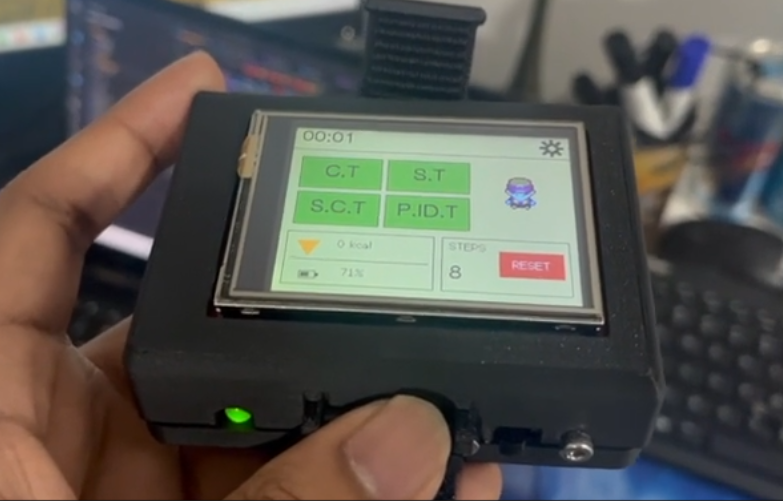
\includegraphics[width=0.55\textwidth]{product.png}}     
    \caption{Lumostep GUI}
\end{figure}
\onecolumn

\section{System Block Diagram}
\begin{figure*}[ht]
    \centering
    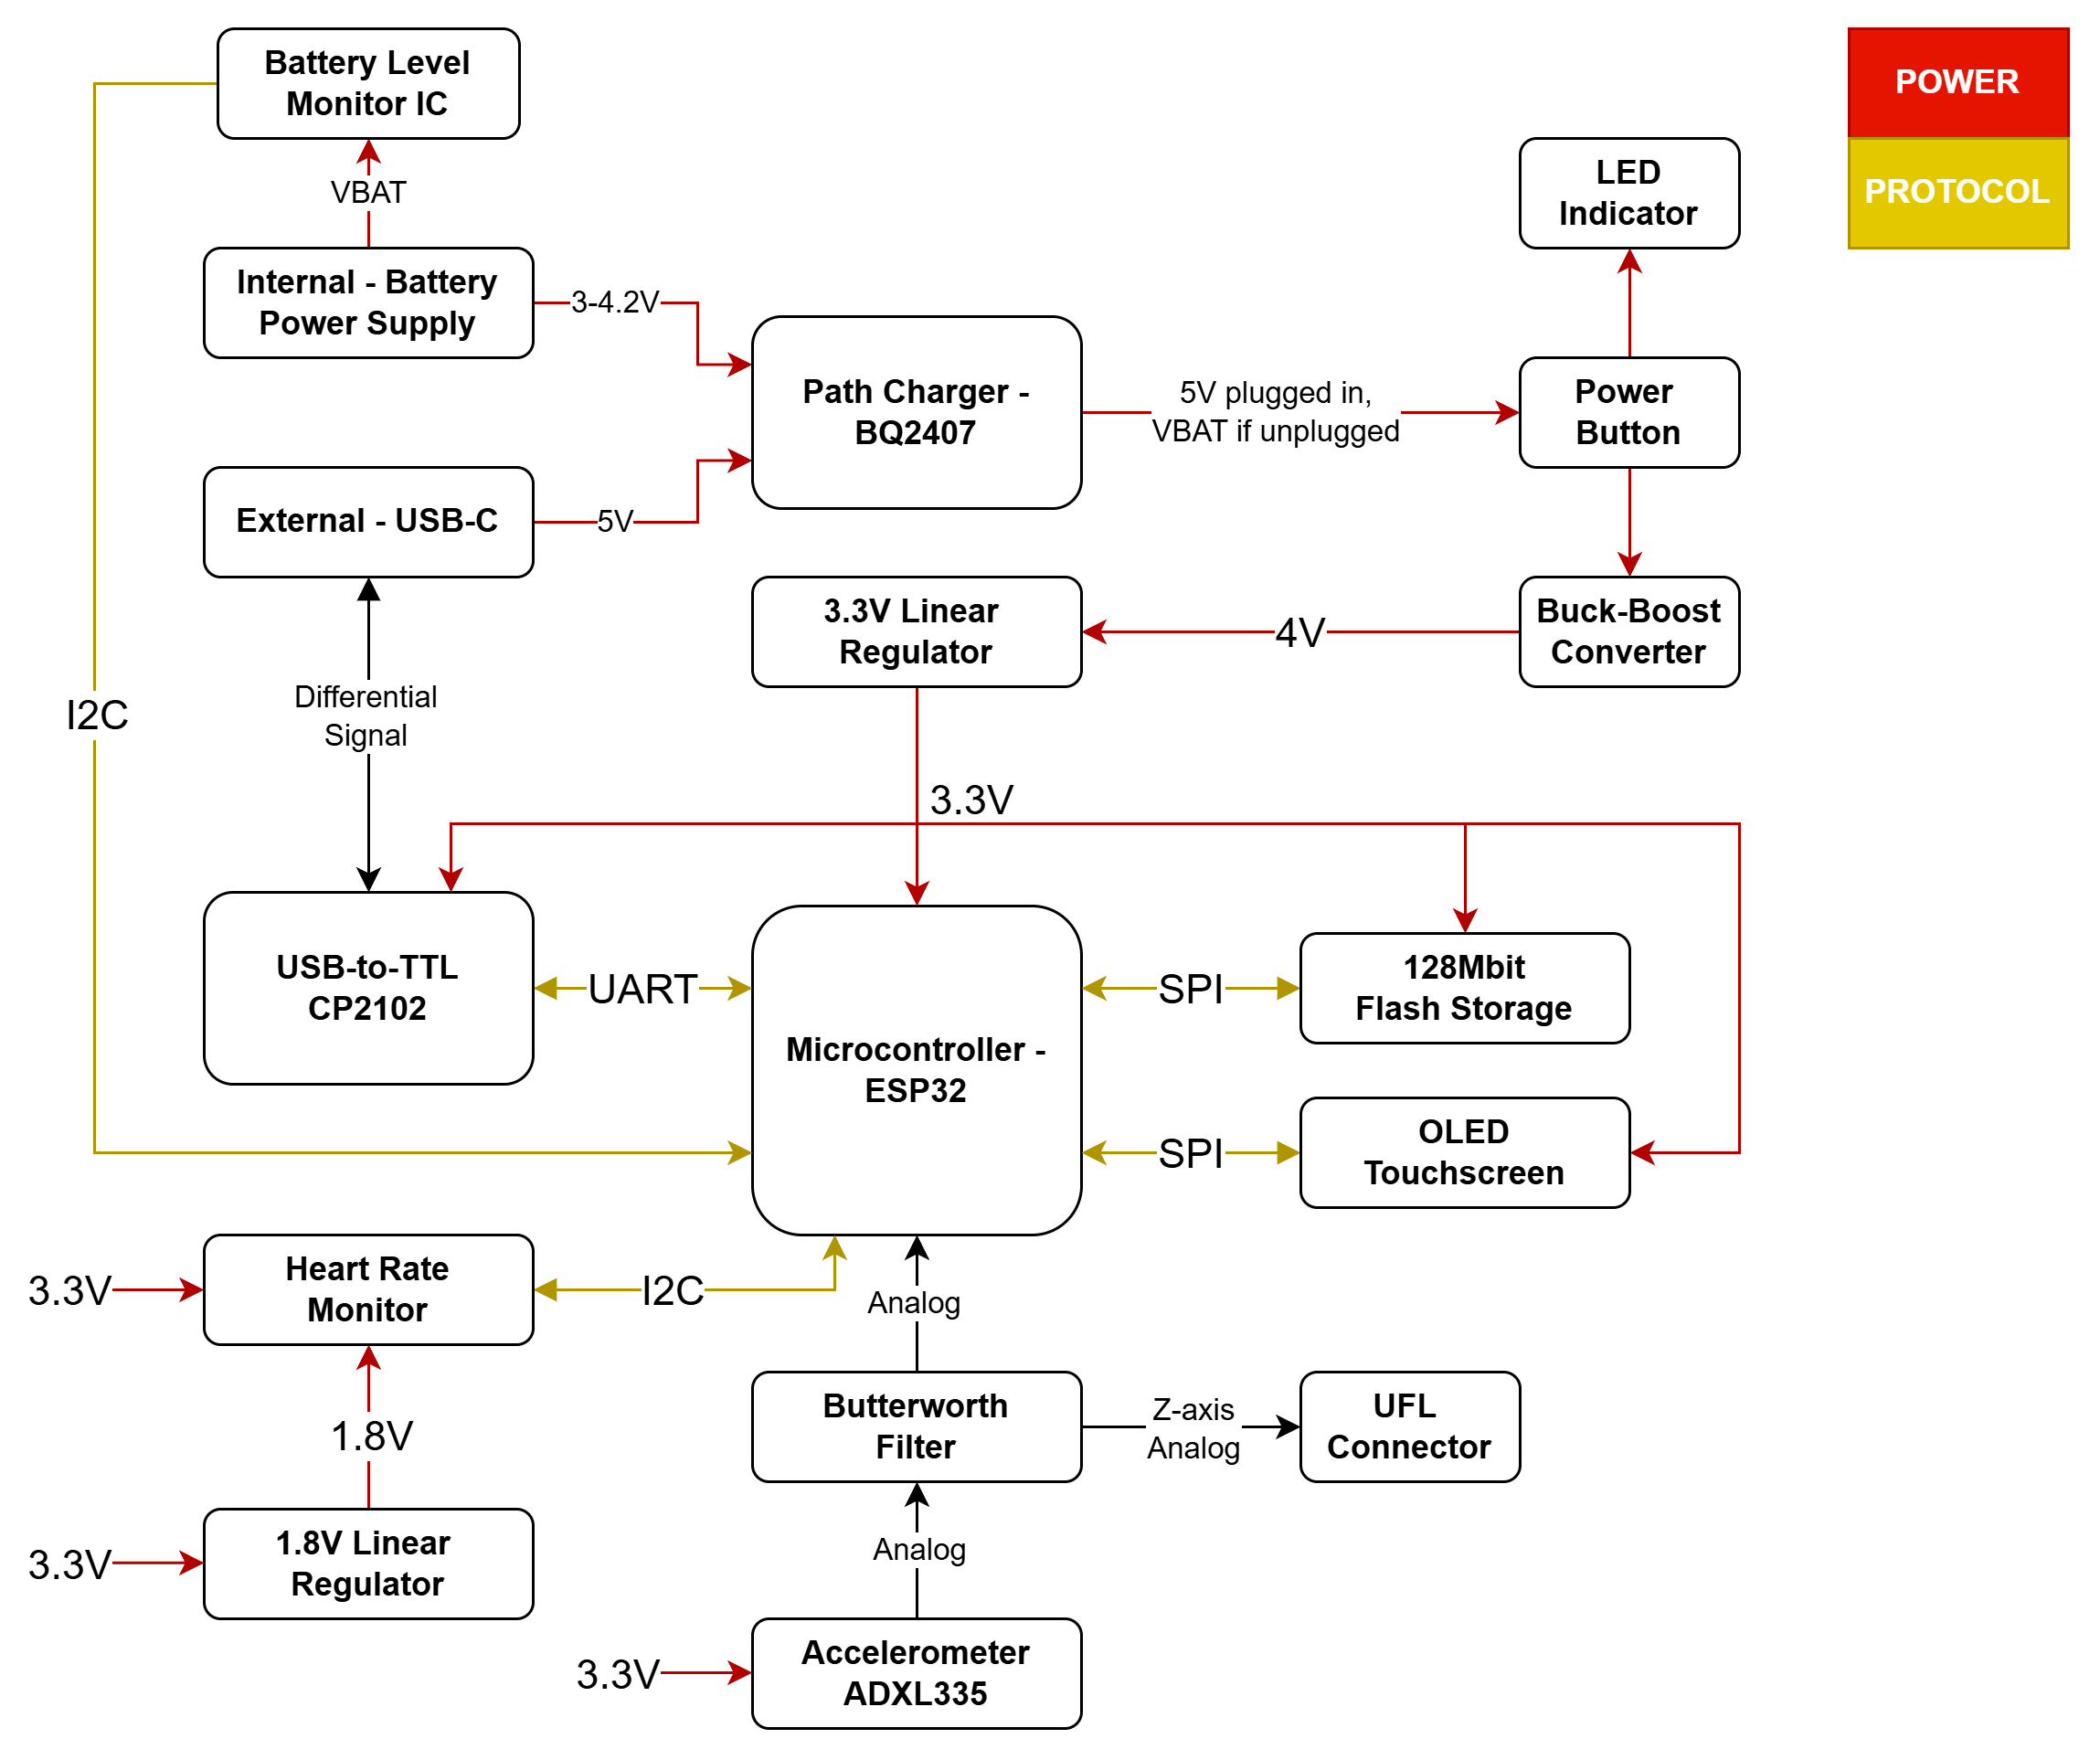
\includegraphics[width=1\textwidth]{dia3.png}
    \caption{Lumostep High-Level System Diagram}
\end{figure*}

% For wide tables, a single column layout is better. It can be switched
% page-by-page.
\section{Signal Mapping}

\begin{longtable}{c | l | l | >{\raggedright\arraybackslash}p{4.5cm} | c}
    \caption{Signal Mapping Table} \label{tab:signalmap} \\
    \thickhline
    \textbf{No.} & \textbf{Source Pin} & \textbf{Signal Name} &
    \textbf{Destination Pin} & \textbf{Direction} \\
    \thickhline
    \endfirsthead

    \multicolumn{5}{l}{\textit{Table \ref{tab:signalmap} continued from previous page}} \\
    \thickhline
    \textbf{No.} & \textbf{Source Pin} & \textbf{Signal Name} &
    \textbf{Destination Pin} & \textbf{Direction} \\
    \thickhline
    \endhead

    \thickhline
    \multicolumn{5}{r}{\textit{Continued on next page}} \\
    \endfoot

    \thickhline
    \endlastfoot

    1  & ESP.GPIO2       & GPIO2/DC         & OLED.D/C                 & Output \\
    2  & ESP.MTCK        & GPIO13/SDI       & OLED.SDI (MOSI)          & Output \\
    3  & ESP.MTMS        & GPIO14/SCK       & OLED.SCK                 & Output \\
    4  & ESP.MTDO        & GPIO15/CS        & OLED.CS                  & Output \\
    5  & ESP.GPIO19      & GPIO19/SDO       & OLED.SDO (MISO)          & Input  \\
    6  & ESP.GPIO25      & GPIO25/TCK       & OLED.T\_CLK              & Output \\
    7  & ESP.GPIO27      & GPIO27/BL        & OLED.LED                 & Output \\
    8  & ESP.32K\_XP     & GPIO32/TDI       & OLED.T\_DIN              & Output \\
    9  & ESP.32K\_XN     & GPIO33/TCS       & OLED.T\_CS               & Output \\
    10 & ESP.SENSOR\_VP  & GPIO36/PEN       & OLED.T\_IRQ              & Input  \\
    11 & ESP.SENSOR\_VN  & GPIO39/TDO       & OLED.T\_OUT              & Input  \\
    12 & OLED.RESET      & MCUEN            & CP2102.DTR               & Input  \\
    \hline
    13 & ESP.CHIP\_PU    & MCUEN            & CP2102.DTR               & Input  \\
    14 & ESP.GPIO0       & MCUIO0           & CP2102.RTS               & Input  \\
    15 & ESP.U0RXD       & MCURX            & CP2102.TXD               & Input  \\
    16 & ESP.U0TXD       & MCUTX            & CP2102.RXD               & Output \\
    \hline
    17 & ESP.VDET\_1     & FILT-X/34        & ADXL.XOUT                & Input  \\
    18 & ESP.VDET\_2     & FILT-Y/35        & ADXL.YOUT                & Input  \\
    19 & ESP.GPIO26      & FILT-Z/26        & ADXL.ZOUT                & Input  \\
    20 & ESP.GPIO4       & ST-CTRL          & ADXL.ST                  & Output \\
    \hline
    21 & ESP.GPIO5       & ESP\_FUEL\_ALERT & MAX17048G.ALERT          & Input  \\
    22 & ESP.GPIO21      & ESP\_SDA         & MAX17048G.SDA            & Bidirectional \\
    23 & ESP.GPIO22      & ESP\_SCL         & MAX17048G.SCL            & Output \\
    \hline
    24 & ESP.GPIO23      & ESP\_INT1        & MAX30102.INT             & Input  \\
    25 & ESP.GPIO21      & ESP\_SDA         & MAX30102.SDA             & Bidirectional \\
    26 & ESP.GPIO22      & ESP\_SCL         & MAX30102.SCL             & Output \\
    \hline
    27 & ESP.SD\_DATA\_0 & SDO/SD0          & W25Q64.DO (IO1)          & Input  \\
    28 & ESP.SD\_DATA\_1 & SDI/SD1          & W25Q64.DI (IO0)          & Output \\
    29 & ESP.SD\_DATA\_2 & SHD/SD2          & W25Q64.HOLD/RESET (IO3)  & Output \\
    30 & ESP.SD\_DATA\_3 & SWP/SD3          & W25Q64.WP (IO2)          & Output \\
    31 & ESP.SD\_CLK     & SCK/CLK          & W25Q64.CLK               & Output \\
    32 & ESP.SD\_CMD     & SCS/CMD          & W25Q64.CS                & Output \\
    \hline
    33 & CP2102.D-       & D1\_N            & USB4110.Dn1, USB4110.Dn2 & Bidirectional \\
    34 & CP2102.D+       & D1\_P            & USB4110.Dp1, USB4110.Dp2 & Bidirectional \\
\end{longtable}

\section{Hardware Requirements}

{\small
\renewcommand{\arraystretch}{1.3}
\setlength{\tabcolsep}{5pt}

\begin{longtable}{@{} c | >{\raggedright\arraybackslash}p{3.2cm} | c c c | c | >{\raggedright\arraybackslash}p{6.3cm} @{}}
    \caption{Hardware Requirements} \label{tab:hw_req} \\
    \thickhline
    \multirow{2}{*}{\textbf{ID}} & \multirow{2}{*}{\textbf{Name}} &
    \multicolumn{3}{c|}{\textbf{Values}} &
    \multirow{2}{*}{\textbf{Unit}} & \multirow{2}{*}{\textbf{Description}} \\
    \cline{3-5}
    & & \textbf{Min} & \textbf{Typ} & \textbf{Max} & & \\
    \thickhline
    \endfirsthead

    \multicolumn{7}{@{}l}{\textit{Table \ref{tab:hw_req} continued from previous page}} \\
    \thickhline
    \multirow{2}{*}{\textbf{ID}} & \multirow{2}{*}{\textbf{Name}} &
    \multicolumn{3}{c|}{\textbf{Values}} &
    \multirow{2}{*}{\textbf{Unit}} & \multirow{2}{*}{\textbf{Description}} \\
    \cline{3-5}
    & & \textbf{Min} & \textbf{Typ} & \textbf{Max} & & \\
    \thickhline
    \endhead

    \hline
    \multicolumn{7}{r@{}}{\textit{Continued on next page}} \\
    \endfoot

    \thickhline
    \endlastfoot

    \multicolumn{7}{@{}l}{\textit{\textbf{Physical}}} \\[2pt]
    \hline
    HW.1  & Mass                      & -    & -     & 0.75  & kg    & Maximum mass of the device for user comfort. \\   
    HW.2  & Shaker mount              & \multicolumn{3}{c|}{4$\times$ M3 holes} & -     & Enclosure mounts onto the lab mount interface via four M3 screws. \\
    HW.3  & Wall thickness            & 1    & 2     & 4     & mm    & Thickness of the 3D-printed enclosure walls. \\
    HW.4  & Wearable strap            & \multicolumn{3}{c|}{Required}           & -     & Durable strap to attach the device to the user's wrist. \\
    HW.5  & PCB count                 & 1    & 2     & 5     & -     & Number of distinct PCBs in the system. \\
    HW.6  & Board width               & 30   & 50    & 80    & mm    & Width of the main PCB, sized for common wrist dimensions. \\
    HW.7  & Board length              & 30   & 50  & 80    & mm    & Length of the main PCB. \\
    HW.8  & Stack-up thickness        & 13   & 20 & 30    & mm    & Combined thickness of battery, PCB and OLED breakout. \\
    HW.9  & OLED touch display        & 2.0  & 2.4   & 2.8   & inch  & Size of the capacitive-touch OLED. \\
    HW.10 & Operating temperature     & -10  & 25    & 85    & $^{\circ}$C & Temprature range over which the device must remain functional. \\[3pt]

    \multicolumn{7}{@{}l}{\textit{\textbf{Electrical}}} \\[2pt]
    \hline
    HW.11 & Current draw              & -    & -     & 2     & A     & Maximum continuous current consumed by the system. \\
    HW.12 & Operating voltage         & 3.3  & -     & 5     & V     & Supply voltage range. \\
    HW.13 & Battery capacity          & 300  & 500   & 1500  & mAh   & Capacity of the built-in Lipo \\
    HW.14 & Power source              & \multicolumn{3}{c|}{Battery + USB-C}    & -     & Auto-switching power from onboard LiPo and USB-C. \\
    HW.15 & SMD package size          & 0604 & -     & 1206  & -     & Package sizes for capacitor, resistor and inductor for ease of soldering. \\
    HW.16 & ADC resolution            & 8    & 12    & 32    & bit   & Resolution of the ADC reading the ADXL outputs. \\
    HW.17 & ADXL filter cutoff        & 30   & 50 & 100   & Hz    & Low-pass Butterworth cutoff for X, Y, Z. \\
    HW.18 & ADXL test point           & \multicolumn{3}{c|}{BNC connector}      & -     & BNC connector on the filtered Z-axis output. \\
    HW.19 & Charge current            & 50  & 250   & 500  & mA    & LiPo charge current set via BQ24074's ISET resistor. \\
    HW.20 & Onboard flash             & 2    & 8     & -    & MB    & External SPI flash for firmware and assets. \\
    HW.21 & Power indicator LED       & \multicolumn{3}{c|}{Required}           & -     & LED to indicate the system is active. \\
    HW.22 & Power switch              & \multicolumn{3}{c|}{Required}           & -     & Switch to turn system on and off. \\
    HW.23 & USB-C ESD protection      & \multicolumn{3}{c|}{Required}           & -     & TVS protection on USB-C D+/D-/VBUS lines. \\
\end{longtable}
}

\newpage
\section{Functional Requirements}

{\small
\renewcommand{\arraystretch}{1.3}
\setlength{\tabcolsep}{5pt}

\begin{longtable}{@{} c | >{\raggedright\arraybackslash}p{3.2cm} | c c c | c | >{\raggedright\arraybackslash}p{6.3cm} @{}}
    \caption{Functional Requirements} \label{tab:fn_req} \\
    \thickhline
    \multirow{2}{*}{\textbf{ID}} & \multirow{2}{*}{\textbf{Name}} &
    \multicolumn{3}{c|}{\textbf{Values}} &
    \multirow{2}{*}{\textbf{Unit}} & \multirow{2}{*}{\textbf{Description}} \\
    \cline{3-5}
    & & \textbf{Min} & \textbf{Typ} & \textbf{Max} & & \\
    \thickhline
    \endfirsthead

    \multicolumn{7}{@{}l}{\textit{Table \ref{tab:fn_req} continued from previous page}} \\
    \thickhline
    \multirow{2}{*}{\textbf{ID}} & \multirow{2}{*}{\textbf{Name}} &
    \multicolumn{3}{c|}{\textbf{Values}} &
    \multirow{2}{*}{\textbf{Unit}} & \multirow{2}{*}{\textbf{Description}} \\
    \cline{3-5}
    & & \textbf{Min} & \textbf{Typ} & \textbf{Max} & & \\
    \thickhline
    \endhead

    \hline
    \multicolumn{7}{r@{}}{\textit{Continued on next page}} \\
    \endfoot

    \thickhline
    \endlastfoot

    \multicolumn{7}{@{}l}{\textit{\textbf{Core behaviour}}} \\[2pt]
    \hline
    FN.1  & ADXL self-test routine        & \multicolumn{3}{c|}{Required}     & -    & Firmware to set the ST pin and verifies the expected output shift on each axis. \\
    FN.2  & ADXL calibration              & \multicolumn{3}{c|}{Required}     & -    & Maps accelerometer output against static gravity; result stored to flash and displayed. \\
    FN.3  & Step counting                 & \multicolumn{3}{c|}{Required}     & -    & Detects steps from filtered accelerometer readings. \\
    FN.4  & Walking pace identification       & \multicolumn{3}{c|}{Required}     & -    & Estimates walking pace (stand, walk, run) from step frequency and magnitude. \\
    FN.5  & GUI display                   & \multicolumn{3}{c|}{Required}     & -    & GUI on the OLED for launching subroutines and showing readings. \\
    FN.6  & Calorie tracking              & \multicolumn{3}{c|}{Optional}     & -    & Estimates kcal from the user's weight and pace. \\
    FN.7  & Firmware update via USB-C     & \multicolumn{3}{c|}{Required}     & -    & Flashing over USB-C without pressing Boot, using CP2102 auto-reset. \\[3pt]

    \multicolumn{7}{@{}l}{\textit{\textbf{Performance}}} \\[2pt]
    \hline
    FN.8  & \texttt{loop()} execution     & -   & -     & 2000  & ms   & Duration of one main-loop iteration. \\
    FN.9  & Step count accuracy           & -    & $\pm$5 & $\pm$10 & \%  & Error vs.\ ground truth over a 100-step walk. \\
    FN.10 & Battery life (active)         & 2    & 6    & -     & h    & Continuous use with display on and step counting active. \\
    FN.11 & Charge time (0\,$\to$\,100\%) & -    & 2     & 4     & h    & Empty-to-full over USB-C at typical charge current. \\
    FN.12 & Boot time                     & -    & 2     & 5     & s    & Power-on to usable GUI. \\
    FN.13 & Touch latency                 & -    & 50    & 100   & ms   & Delay between touch event and GUI update. \\
\end{longtable}
}
\section{Schematic Designs}
The Lumostep PCB is designed and laid out in Altium, with 9 subcircuits covering different systems. Refer to the following figures for more details.
\newpage
\begin{landscape}

% --- Main content ---
\begin{figure}
    \centering
    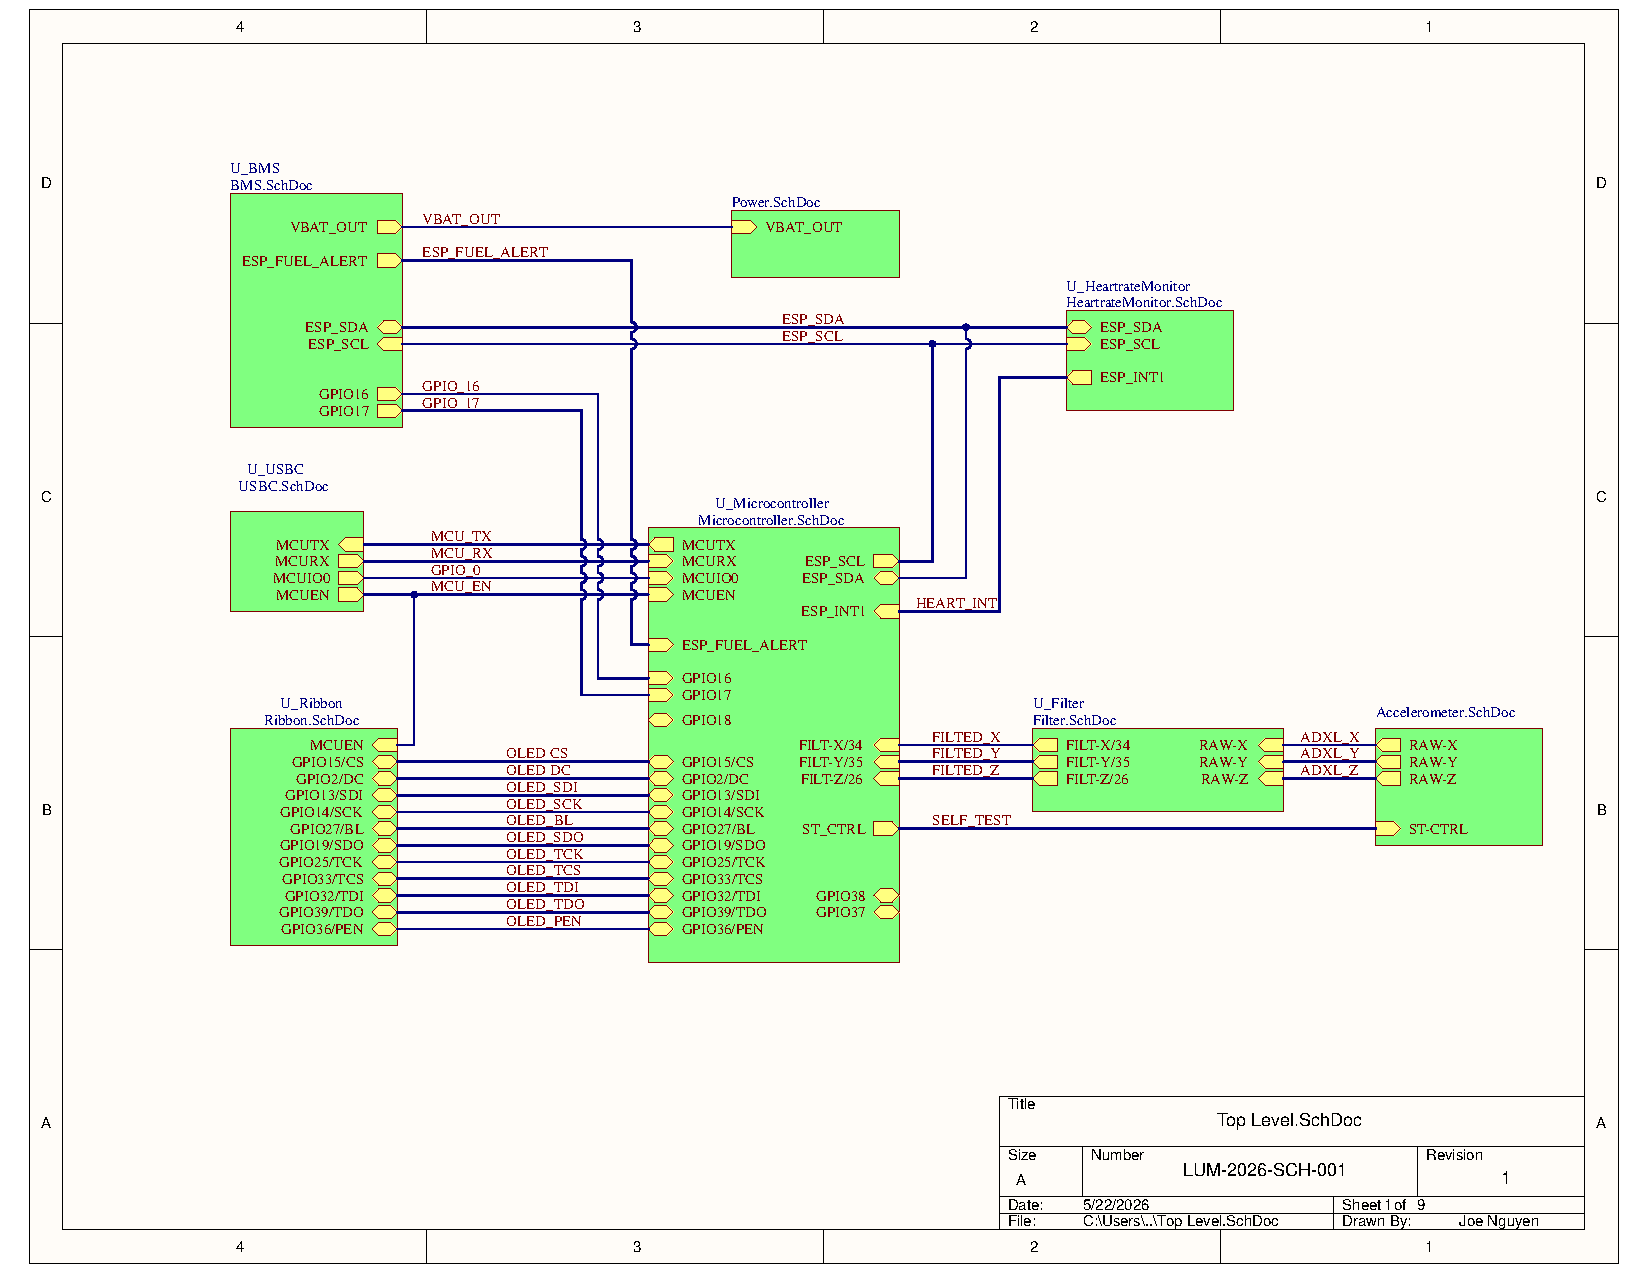
\includegraphics[width=\linewidth, keepaspectratio]{Top Level.pdf}
    \caption{Lumostep top-level schematic}
\end{figure}

\begin{figure}
    \centering
    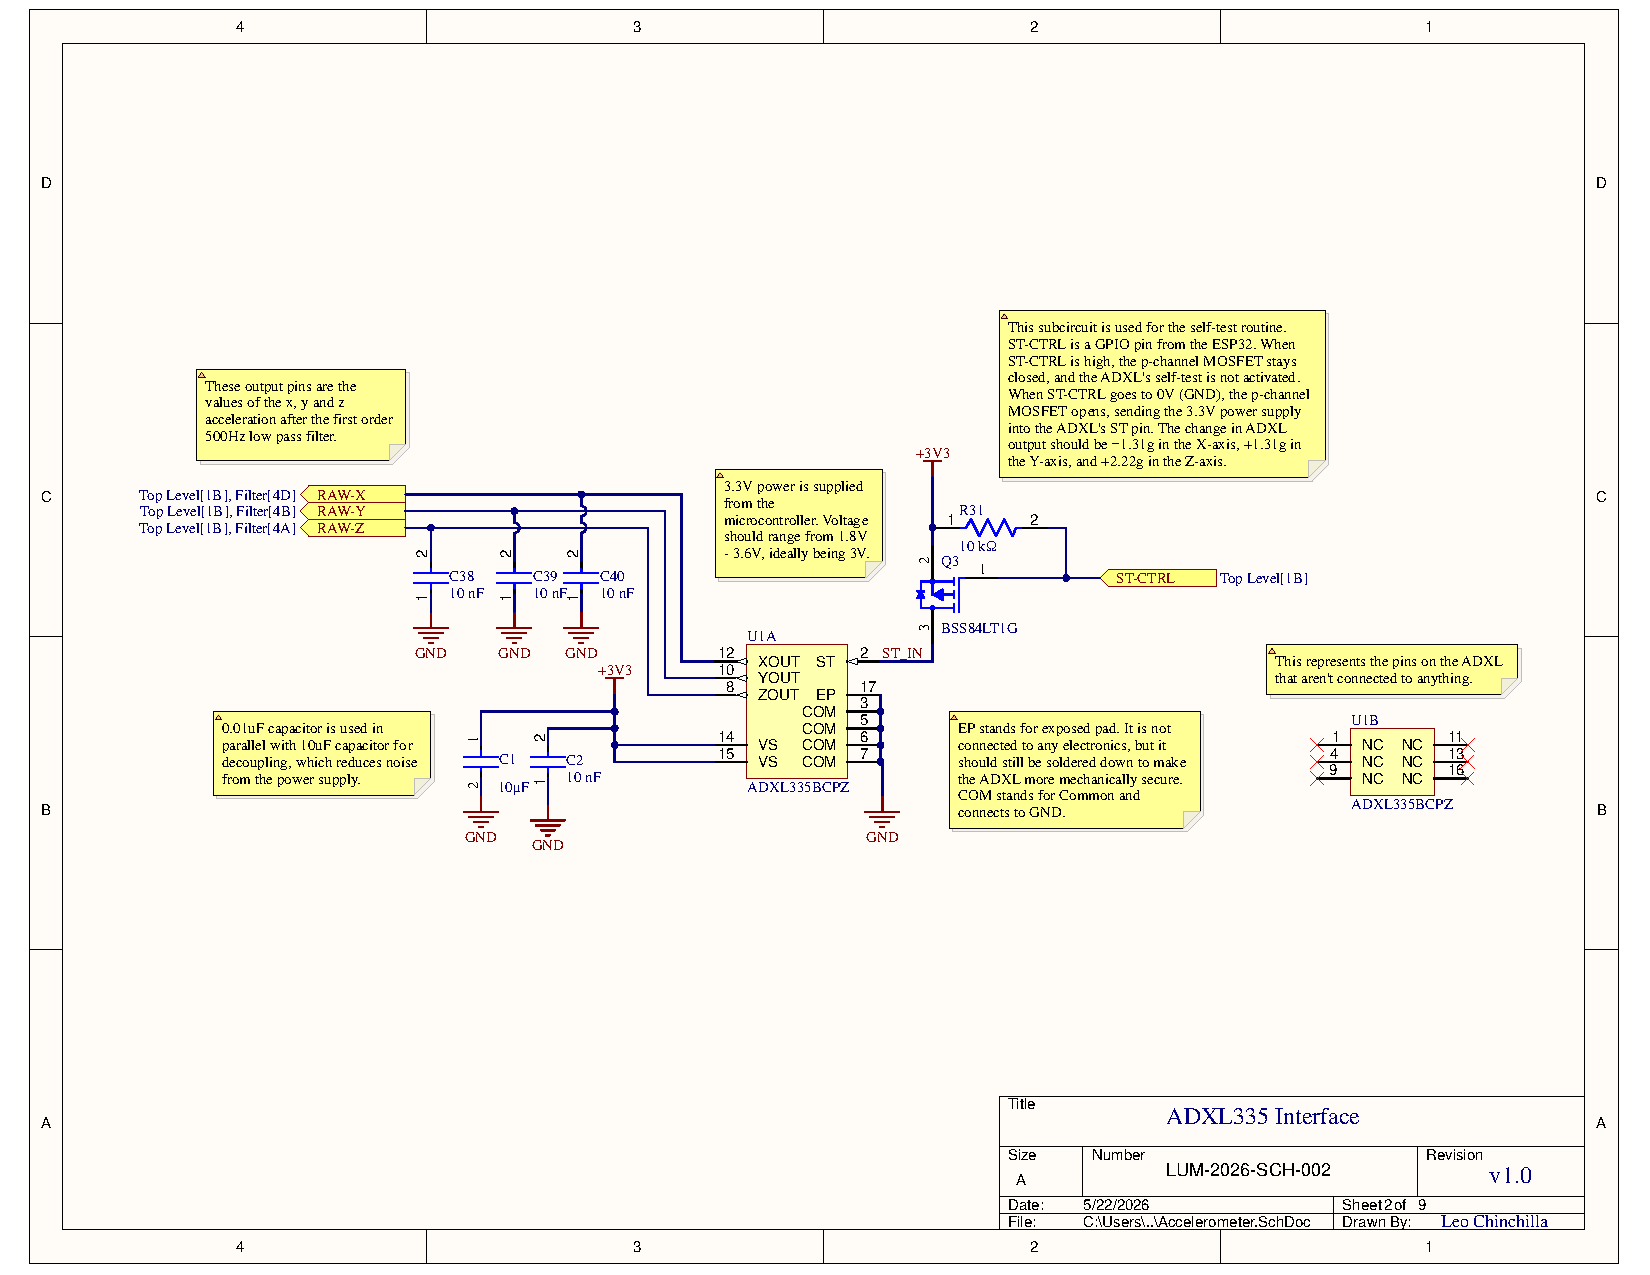
\includegraphics[width=\linewidth, keepaspectratio]{Accelerometer.pdf}
    \caption{Lumostep ADXL335 Interface Subcircuit}
\end{figure}

\begin{figure}
    \centering
    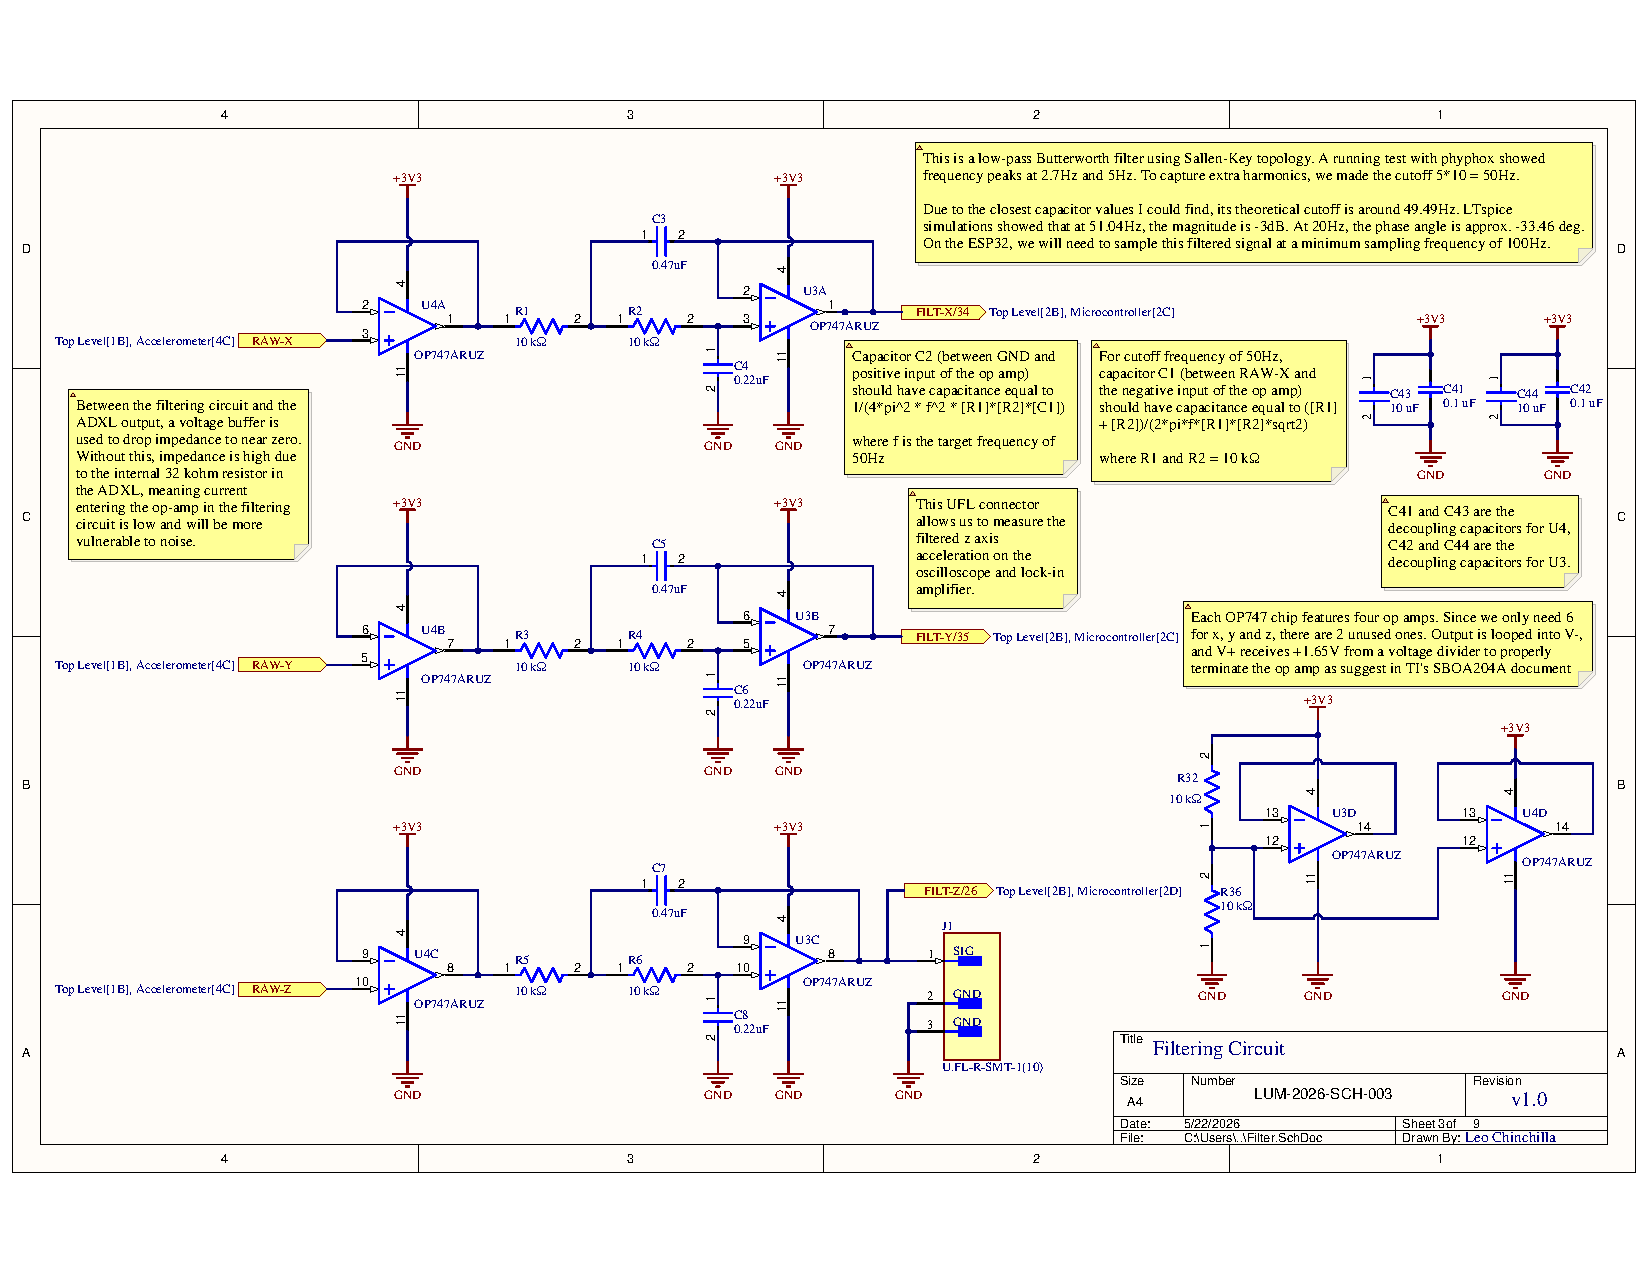
\includegraphics[width=\linewidth, keepaspectratio]{Filter.pdf}
    \caption{Lumostep ADXL335 Analog Filtering Subcircuit}
\end{figure}

\begin{figure}
    \centering
    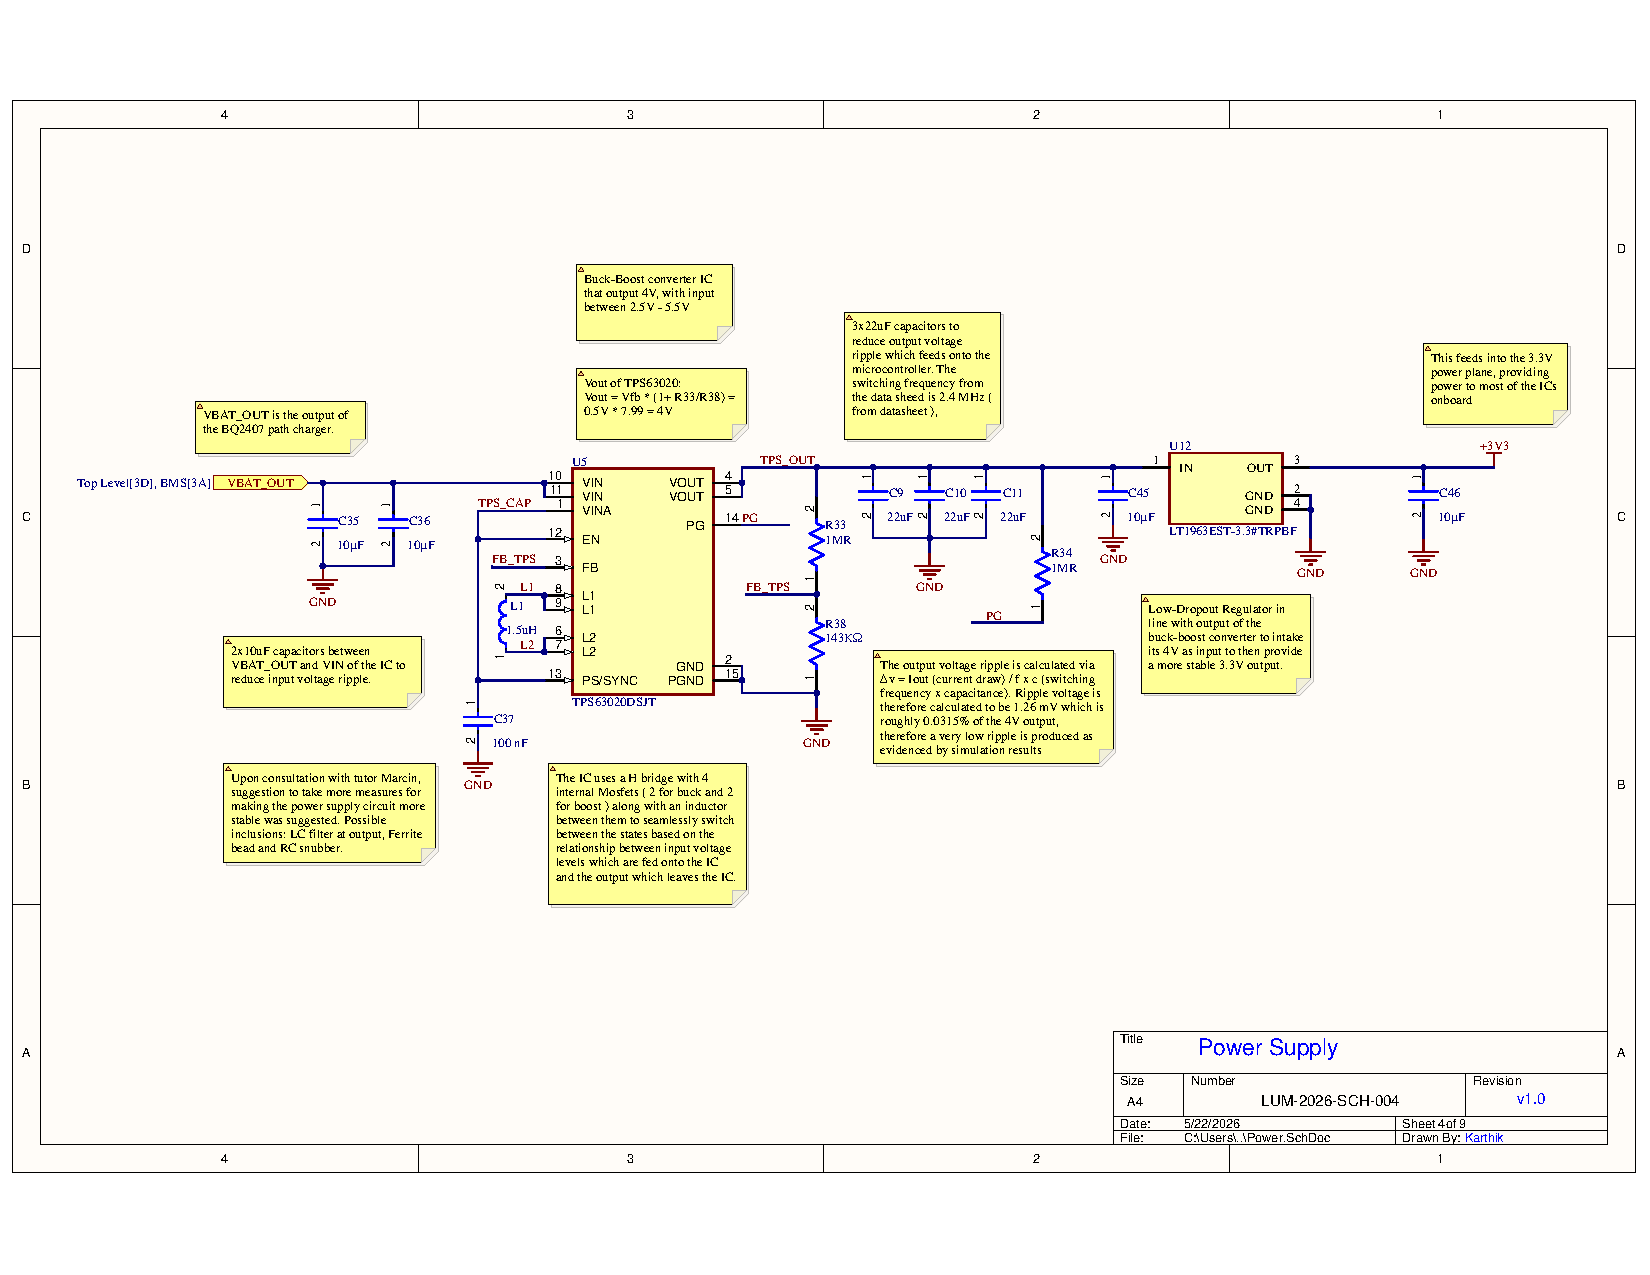
\includegraphics[width=\linewidth, keepaspectratio]{Power.pdf}
    \caption{Lumostep ADXL335 Power Supply Subcircuit}
\end{figure}

\begin{figure}
    \centering
    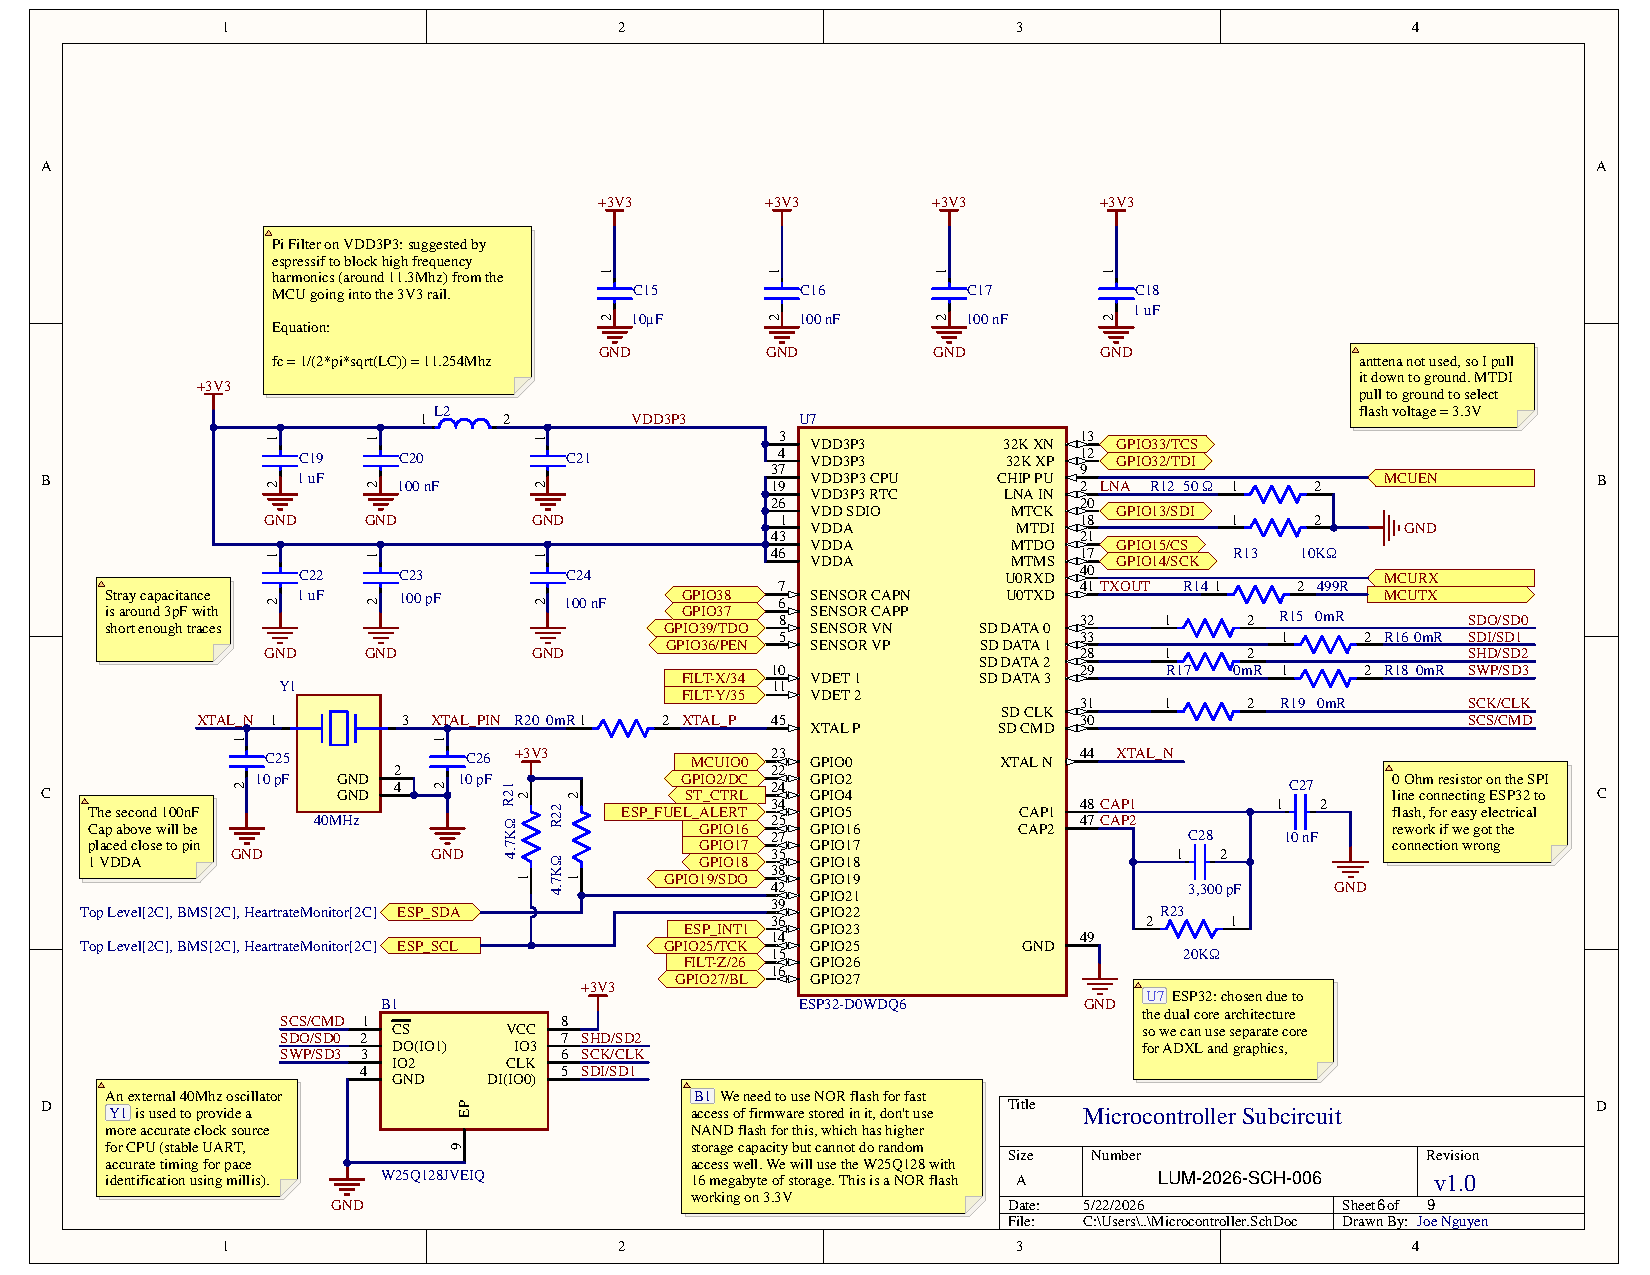
\includegraphics[width=\linewidth, keepaspectratio]{Microcontroller.pdf}
    \caption{Lumostep Main System Microcontroller Subcircuit}
\end{figure}

\begin{figure}
    \centering
    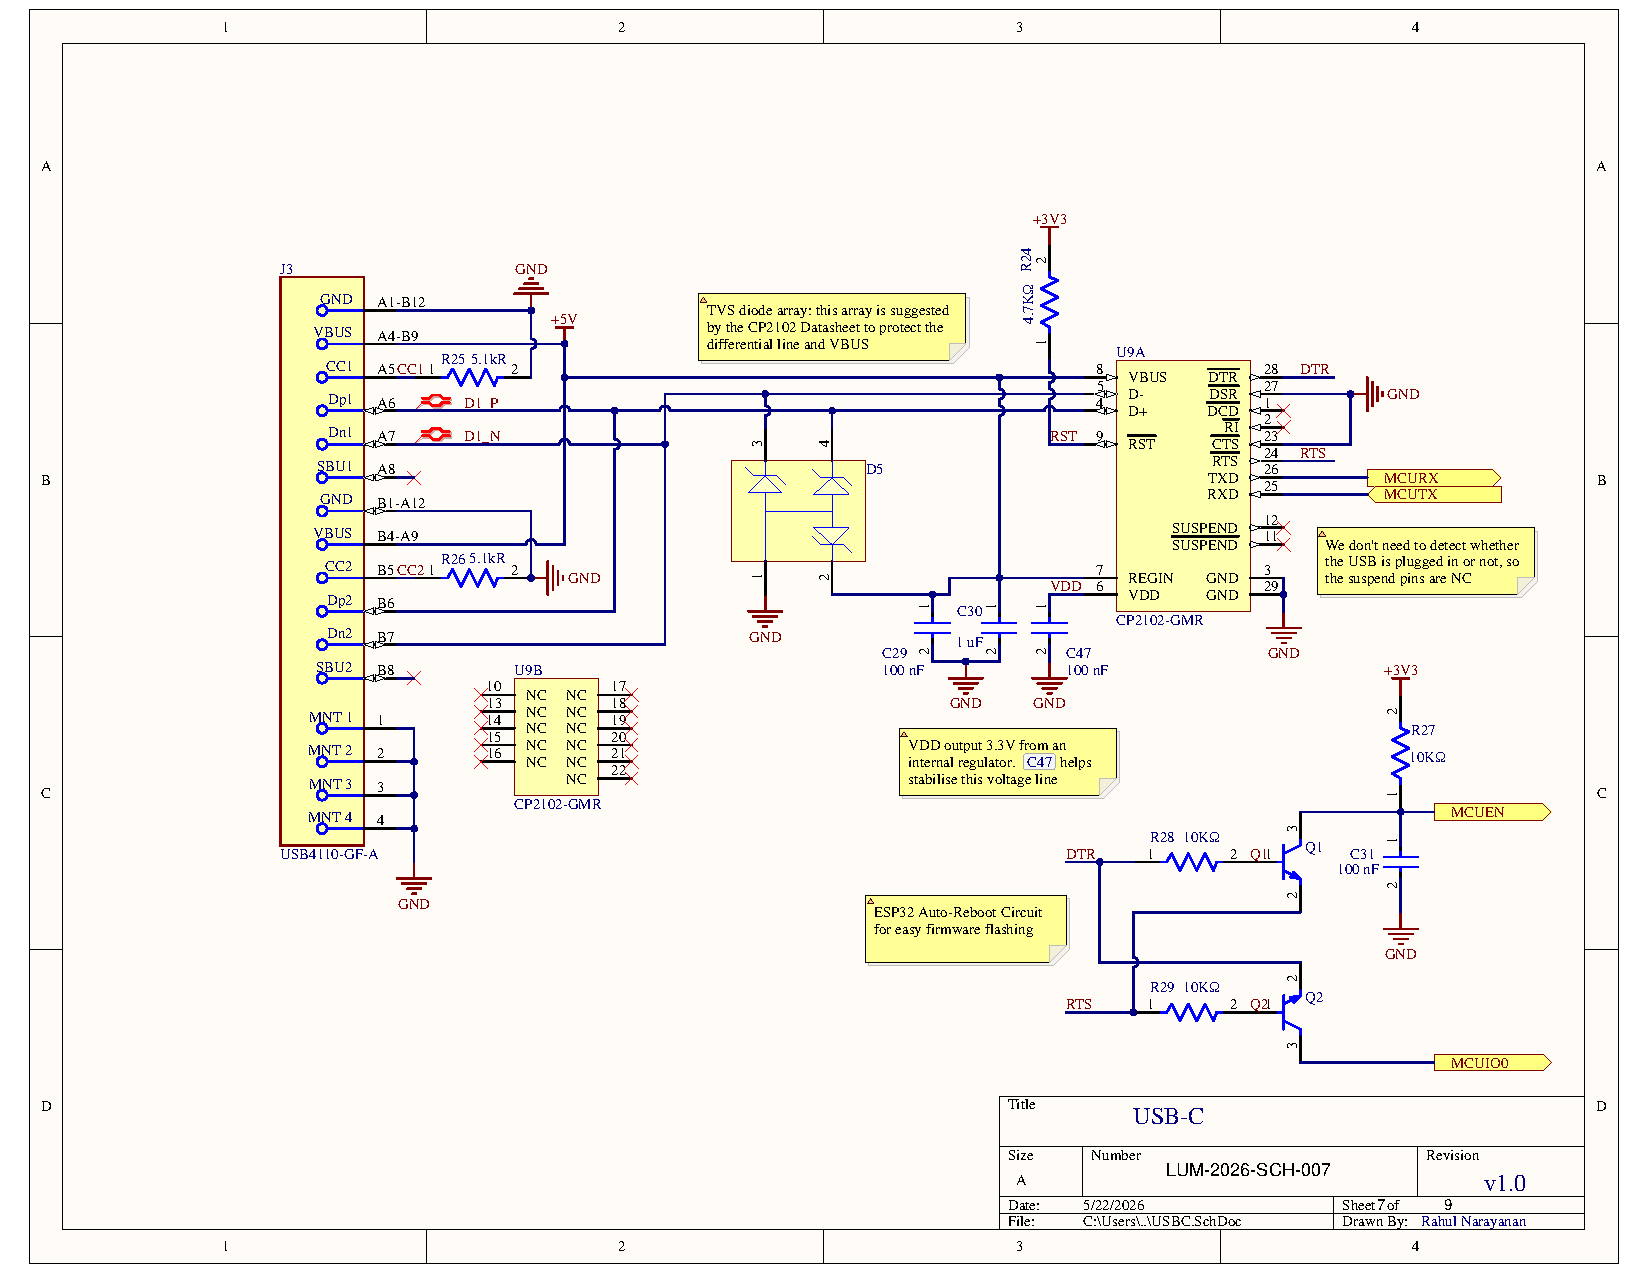
\includegraphics[width=\linewidth, keepaspectratio]{USBC.pdf}
    \caption{Lumostep USB-C Power Delivery and ESP32 Communication Subcircuit}
\end{figure}

\begin{figure}
    \centering
    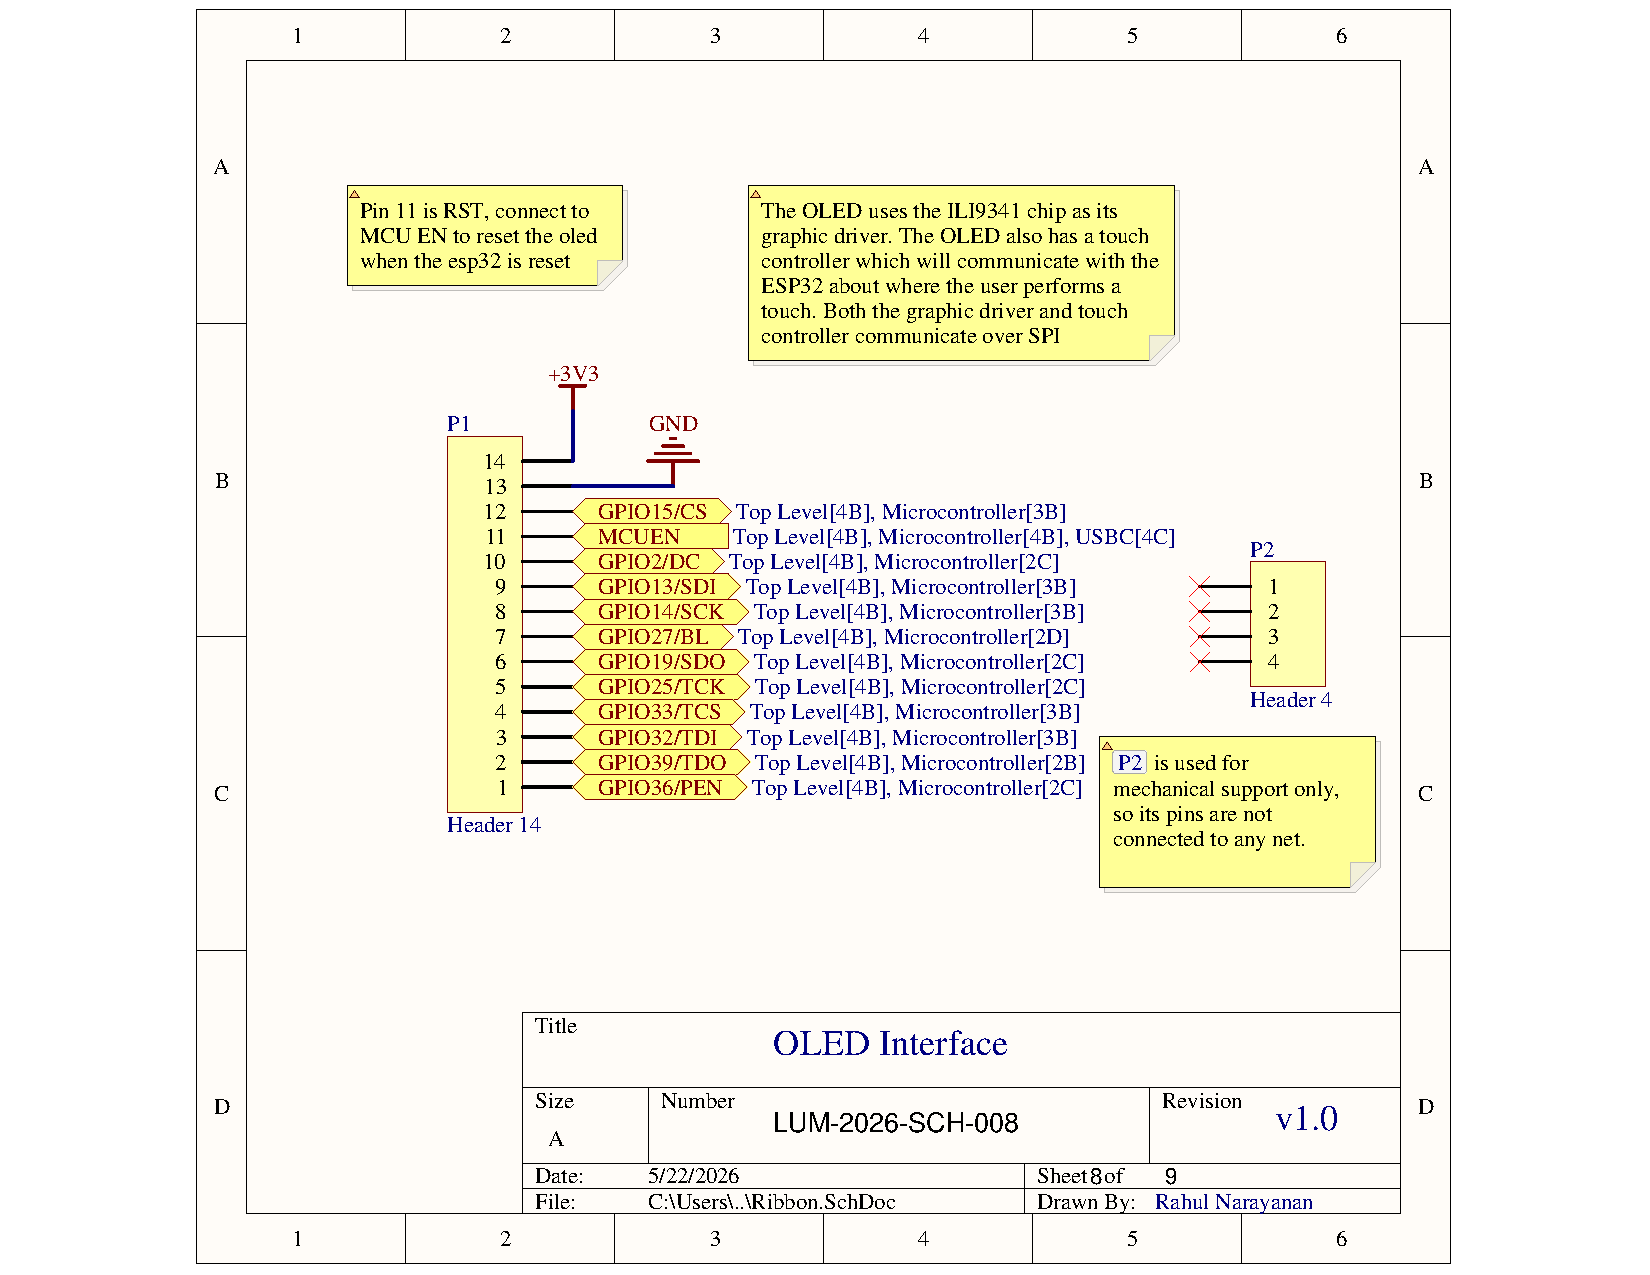
\includegraphics[width=\linewidth, keepaspectratio]{Ribbon.pdf}
    \caption{Lumostep OLED Interface Subcircuit}
\end{figure}

\begin{figure}
    \centering
    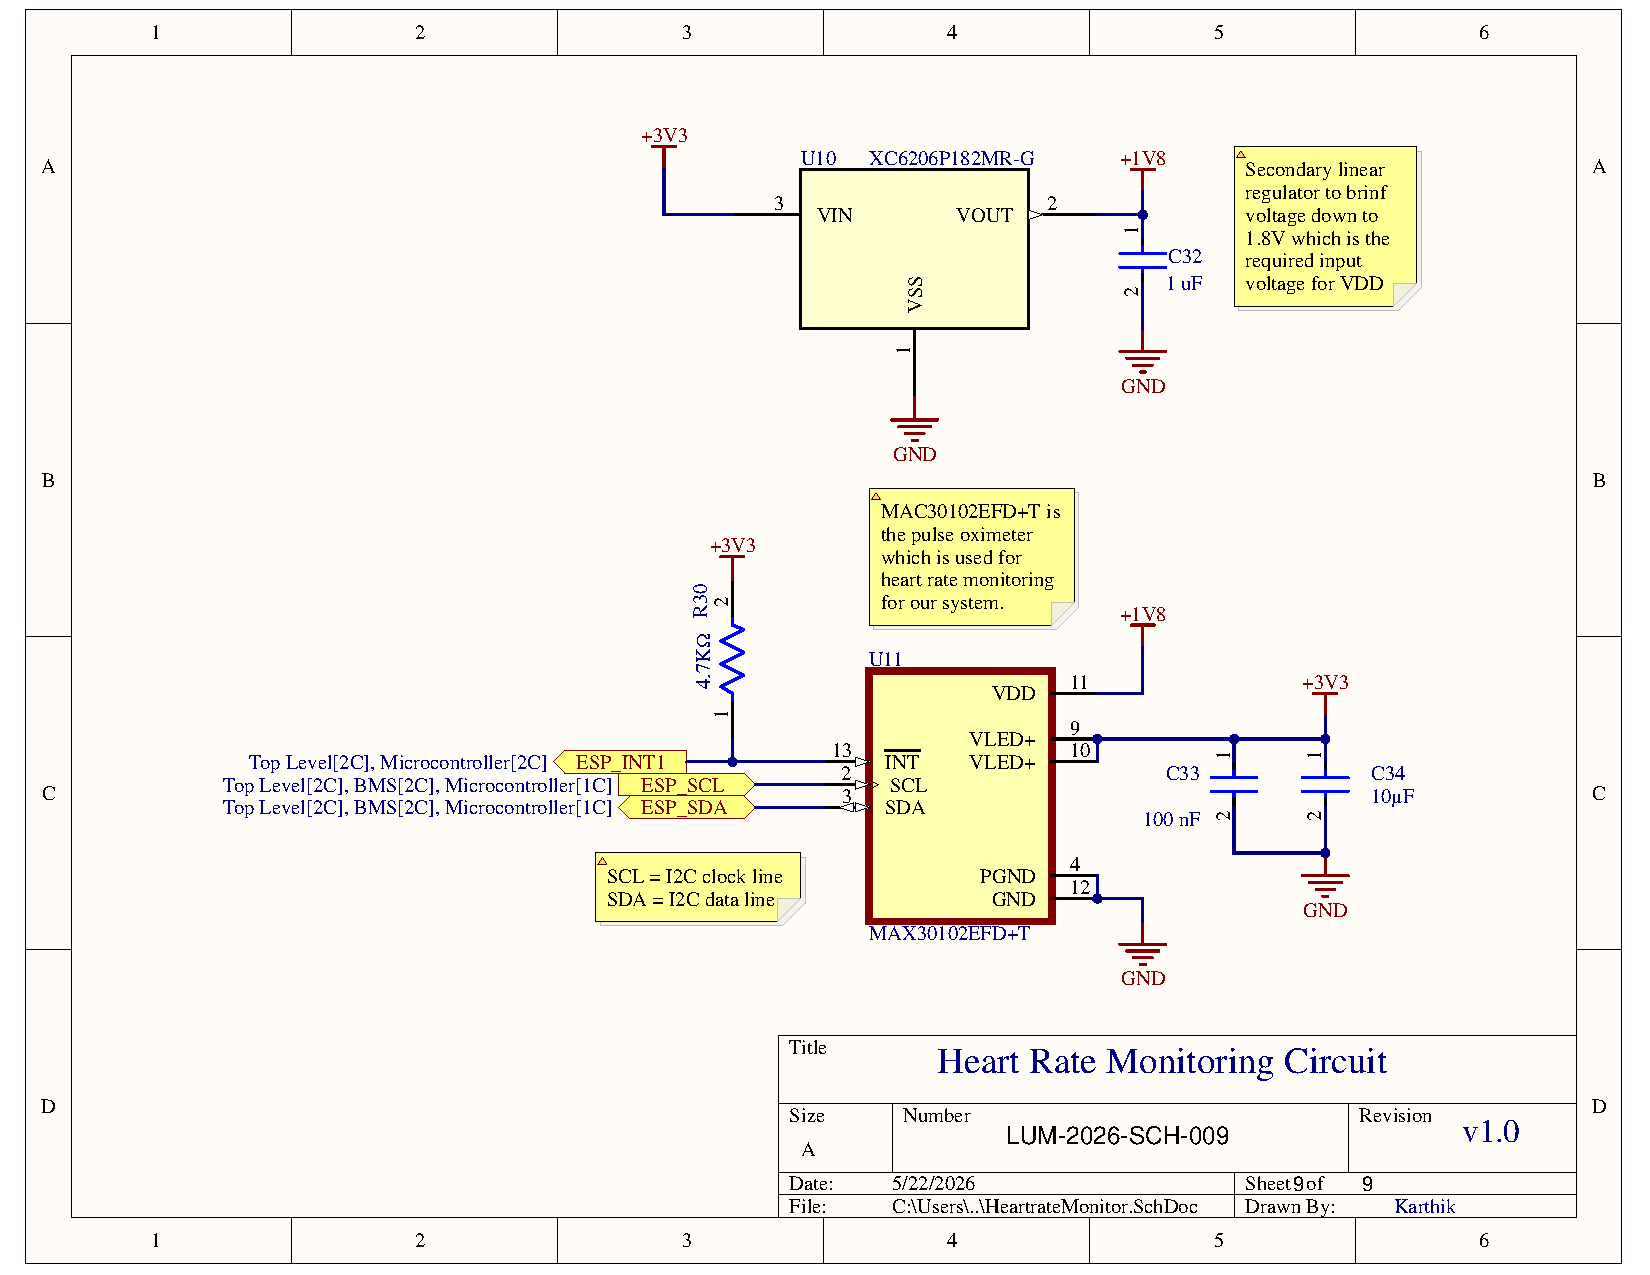
\includegraphics[width=\linewidth, keepaspectratio]{HeartrateMonitor.pdf}
    \caption{Lumostep Heart Rate Monitoring Subcircuit}
\end{figure}

\end{landscape}
\end{document}

